\documentclass[10pt,a4paper]{article}
\usepackage[margin=2cm]{geometry}
\usepackage{graphicx,booktabs,amsmath,xcolor,hyperref,caption,float}
\usepackage[numbers,sort&compress]{natbib}
\captionsetup{font=small,labelfont=bf}
\setlength{\parskip}{3pt}\setlength{\parindent}{0pt}
\graphicspath{{../results/figures/}}
\newcommand{\TestAcc}{90.9\%}
\newcommand{\ECE}{0.011}
\newcommand{\ConfOK}{0.95}
\newcommand{\ConfBad}{0.67}


\title{\vspace{-1.2cm}\textbf{Learned Scheduler Selection for Disk Scheduling\\under Workload Shift}\\[2pt]
\large CSE-307 Operating Systems --- Term Paper, Section B, Track 2}
\author{Name: Lt Sami}
\author{Student ID: 202314210}
\date{\today}

\begin{document}\maketitle\vspace{-0.6cm}

\begin{abstract}\noindent
No single disk-scheduling policy minimises seek distance for every request pattern
\cite{teorey1972,worthington1994}. I implement FCFS, SSTF, SCAN and C-SCAN, and add a
depth-4 decision tree that inspects a 40-request window and predicts which policy will give
the least head movement, together with a confidence score. On held-out windows the selector
picks the best policy \TestAcc{} of the time and is well calibrated (ECE $=\ECE$; mean confidence
\ConfOK{} when right vs.\ \ConfBad{} when wrong). On a timeline that shifts
sequential$\rightarrow$random$\rightarrow$bursty, a selector trained on all three regimes tracks the
oracle, while a selector that never saw bursty traffic stays $>$95\% confident yet is wrong on
almost every bursty window, nearly tripling seek distance in that phase. Finally, the same
benchmark is run inside an Ubuntu guest on VMware under different RAM/vCPU settings to observe
paging and CPU-scheduling effects.
\end{abstract}

\section{Problem Framing}
A disk scheduler decides the order in which pending requests are served; with mechanical
disks, the dominant cost is moving the arm, so total head movement (cylinders) is the usual
proxy for seek time \cite{silberschatz2018,ostep}. FCFS is fair but ignores geometry; SSTF is
greedy and can starve far requests; SCAN and C-SCAN sweep the arm to bound waiting time
\cite{silberschatz2018}. Which is best depends on the workload: a sequential stream is already
in good order, random traffic rewards geometric reordering, and bursty traffic around hotspots
rewards greedy locality. Real systems see such patterns change after deployment, which is a
\emph{dataset shift} for any learned component \cite{quinonero2009}. The questions studied are:
(Q1) can a lightweight model choose the right policy per window; (Q2) is its confidence
trustworthy; (Q3) what happens to the classical policies and to the model when the workload
shifts.

\section{Implementation}
\textbf{Classical algorithms} (\texttt{src/schedulers.py}) operate on cylinders 0--4999 and
return the service order and total head movement. SCAN sweeps upward to the last cylinder and
reverses; C-SCAN sweeps upward, returns to cylinder~0, and the return jump is counted, following
the textbook example \cite{silberschatz2018}. Unit tests reproduce the textbook queue
(head 53; FCFS 640, SSTF 236, SCAN 236, C-SCAN 382 cylinders).

\textbf{Learned selector} (\texttt{src/selector.py}). Each window of 40 requests is described by
six cheap features: normalised standard deviation of track positions, mean jump between
consecutive arrivals (a burstiness/locality measure), fraction of increasing steps
(monotonicity), span, offset of the mean request from the head, and number of separated
clusters. The label is the policy with the smallest head movement for that window (ties go to
FCFS, the cheapest to run). A CART decision tree \cite{breiman1984} (scikit-learn
\cite{sklearn}; max depth 4, $\geq$20 samples per leaf) is trained on 3000 labelled windows. A
tree was chosen because it is tiny, explainable (\texttt{results/decision\_tree.txt}) and costs
only a few comparisons per decision, in the spirit of learned OS/data-system components
\cite{kraska2018}. \textbf{Confidence} is the class fraction in the reached leaf; calibration is
measured with a reliability diagram and expected calibration error (ECE) \cite{guo2017}.

\section{Experimental Setup}
\textbf{Workloads} (\texttt{src/workload.py}): \emph{sequential} (increasing cylinders with small
jitter, continuing from the previous window), \emph{random} (uniform), and \emph{bursty}
(bursts of 3--8 requests around 2--3 hotspots, interleaved). \textbf{E1:} train on 1000
windows/type (seed 1), test on 500 windows/type (seed 2) with random head positions.
\textbf{E2 (shift):} 120 consecutive windows: 40 sequential, 40 random, 40 bursty; each policy
carries its own head position between windows. Besides the full selector, a
\emph{shift-naive} selector trained only on sequential+random windows is evaluated, to isolate
the effect of an unseen regime. An oracle (best policy per window) gives the lower bound.
\section{Results}
\begin{table}[H]\centering\small
\caption{E1: mean head movement per 40-request window on the test set (cylinders; lower is better).}
\begin{tabular}{lrrrrrr}\toprule
 & FCFS & SSTF & SCAN & C-SCAN & Selector & Oracle\\\midrule
bursty & 10,569 & 3,210 & 5,084 & 7,353 & 3,210 & 3,202\\
random & 66,423 & 6,994 & 7,216 & 9,776 & 6,642 & 6,517\\
sequential & 800 & 910 & 2,710 & 5,372 & 800 & 800\\
all & 25,930 & 3,705 & 5,004 & 7,500 & 3,550 & 3,506\\
\bottomrule\end{tabular}
\end{table}
\vspace{-6pt}
\textbf{E1.} SSTF is the best single policy overall, but not everywhere: on sequential windows
FCFS is better because the arrival order is already near-optimal and SSTF's greedy choice can
step backwards to a jittered request; on random windows SCAN occasionally beats SSTF when the
head is near one side. C-SCAN never wins on seek distance (its return jump is pure cost; its
benefit is uniform waiting time, which this metric does not reward). Exploiting these
differences, the selector reduces mean seek below SSTF (3550 vs.\ 3705 cylinders, $-4.2\%$) and
comes within 1.3\% of the oracle. Accuracy is \TestAcc{} overall (99\% sequential, 99\% bursty,
75\% random); the random-workload errors are mostly SSTF/SCAN near-ties, so they cost little.

\begin{figure}[H]\centering
\begin{minipage}{0.66\linewidth}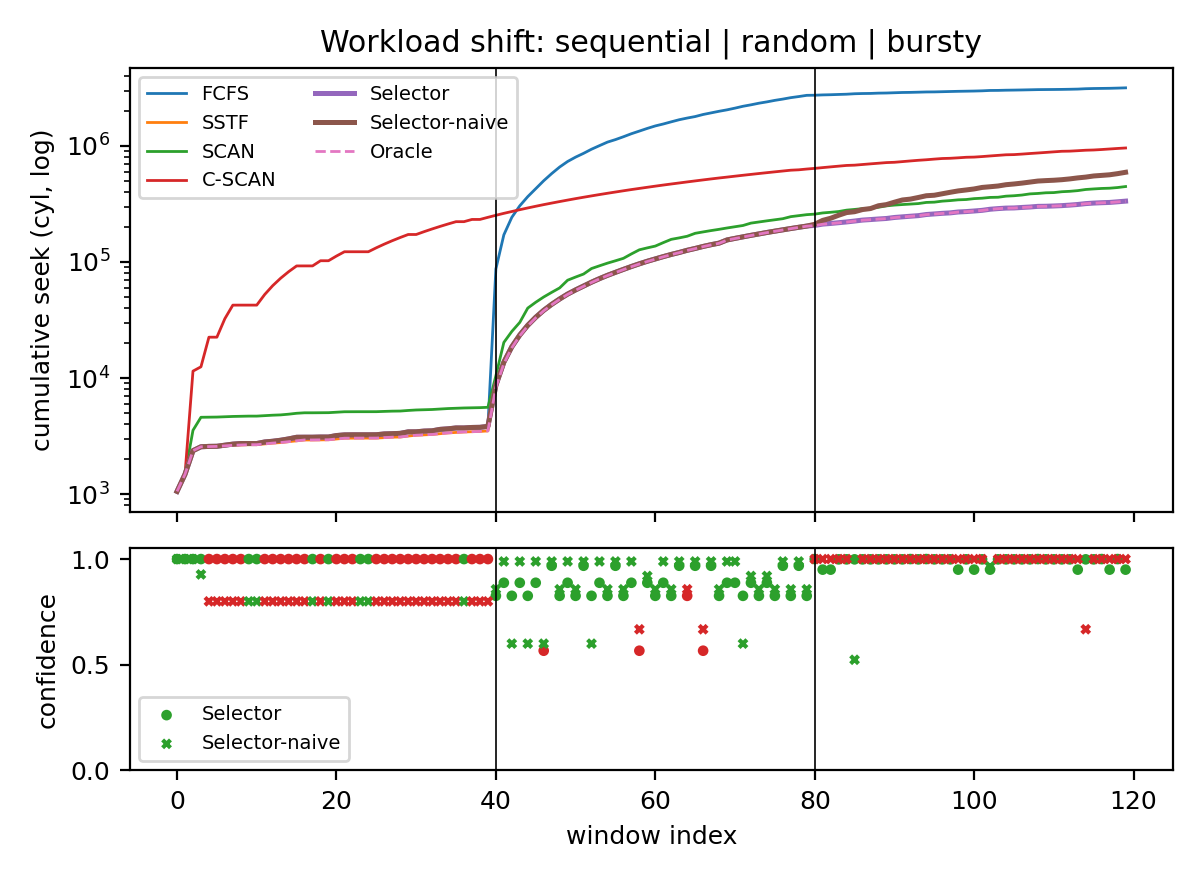
\includegraphics[width=\linewidth]{fig_shift_timeline.png}\end{minipage}\hfill
\begin{minipage}{0.32\linewidth}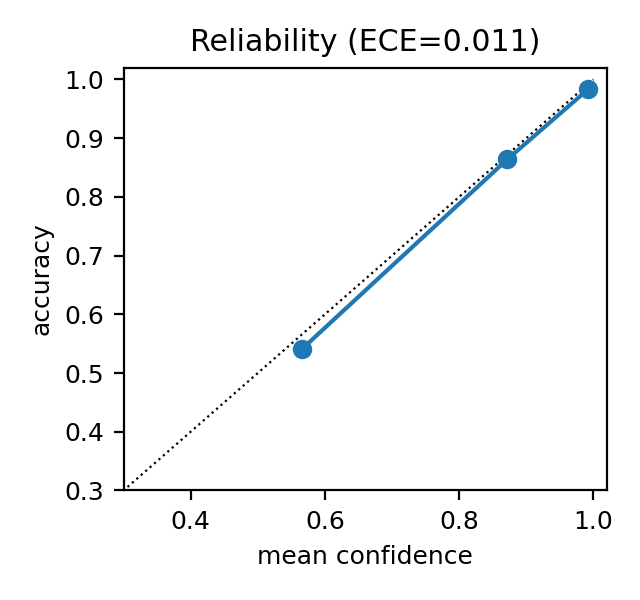
\includegraphics[width=\linewidth]{fig_calibration.png}\end{minipage}
\caption{Left: E2 cumulative head movement (log scale) across the shift (vertical lines) and per-window selector confidence (green = correct, red = wrong). Right: E1 reliability diagram; points near the diagonal mean confidence matches accuracy.}
\end{figure}

\textbf{Calibration (Q2).} In distribution the confidence is meaningful: ECE $=\ECE$, and mean
confidence is \ConfOK{} on correct picks vs.\ \ConfBad{} on wrong ones. Low-confidence leaves
(0.5--0.6) are exactly where random windows have SSTF/SCAN near-ties.

\begin{table}[H]\centering\small
\caption{E2: total head movement per phase of the shift timeline (cylinders).}
\begin{tabular}{lrrrr}\toprule
 & sequential & random & bursty & total\\\midrule
FCFS & 3,834 & 2,722,295 & 436,715 & 3,162,844\\
SSTF & 3,504 & 199,828 & 130,405 & 333,737\\
SCAN & 5,596 & 250,028 & 190,851 & 446,475\\
C-SCAN & 242,431 & 389,340 & 327,643 & 959,414\\
Selector & 3,834 & 200,002 & 130,405 & 334,241\\
Selector-naive & 3,834 & 199,978 & 388,542 & 592,354\\
Oracle & 3,504 & 199,800 & 130,405 & 333,709\\
\bottomrule\end{tabular}
\end{table}
\vspace{-8pt}
\begin{table}[H]\centering\small
\caption{E2: selector accuracy (fraction of windows where it picked the per-window best) and mean confidence per phase.}
\begin{tabular}{lrrrrrr}\toprule
 & sequential acc & random acc & bursty acc & sequential conf & random conf & bursty conf\\\midrule
Selector & 0.28 & 0.90 & 1.00 & 1.00 & 0.85 & 0.99\\
Selector-naive & 0.28 & 0.93 & 0.05 & 0.82 & 0.88 & 0.98\\
\bottomrule\end{tabular}
\end{table}

\textbf{E2 (Q3).} When traffic switches from sequential to random, FCFS degrades the most (from
3.8k to 2.7M cylinders, about 13.6$\times$ SSTF) because it keeps serving requests in arrival
order across the whole disk. C-SCAN is worst in the sequential phase (each window ends with a
full return sweep) but relatively more stable afterwards. SSTF is robust in all three phases.
The full selector switches from FCFS to SSTF automatically within the first random window and
finishes within 0.2\% of the oracle overall. In the sequential phase its strict accuracy is only
0.28 because FCFS and SSTF differ by a few cylinders (3834 vs.\ 3504 in total); the cost of these
``errors'' is negligible. The shift-naive selector shows the real danger: in the bursty phase
it keeps choosing FCFS with mean confidence 0.98 while being right on only 5\% of windows,
spending 3.0$\times$ the oracle's head movement. A bursty window has small \emph{span}
locally but large jumps between hotspots, which the naive tree, having never seen this
combination, maps onto the sequential (FCFS) leaves. The confidence score is therefore calibrated
\emph{only within the training distribution}; under shift it is overconfident, matching
observations about model calibration under dataset shift \cite{guo2017,quinonero2009}.

\section{Analysis and Conclusion}
(1) The classical policy that degrades most under the shift is FCFS, because its quality depends
entirely on the arrival order matching the disk layout; SSTF and SCAN, which reorder by
geometry, are much less sensitive. (2) A tiny, interpretable classifier can pick the right
policy per window and beats the best fixed policy by a small but consistent margin, and its
confidence is well calibrated in distribution. (3) That confidence cannot be trusted after an
unseen shift: the most dangerous failure is a confident wrong choice, so a deployed selector
should fall back to a robust default (SSTF here) or retrain when feature statistics drift
outside the training range. (4) In a virtualised guest, the same algorithmic work can be
dominated by memory-management effects: once the working set exceeds guest RAM, paging rather
than computation determines run time. \emph{Limitations:} head movement only (no rotational
latency or queueing delay), batch rather than online scheduling, and synthetic workloads.

\small
\bibliographystyle{unsrtnat}\bibliography{references}
\end{document}
